\documentclass[11pt,twocolumn]{article}

% Packages
\usepackage[utf8]{inputenc}
\usepackage[T1]{fontenc}
\usepackage{times}
\usepackage{graphicx}
\usepackage{booktabs}
\usepackage{amsmath}
\usepackage{amssymb}
\usepackage{hyperref}
\usepackage{xcolor}
\usepackage{algorithm}
\usepackage{algorithmic}
\usepackage{multirow}
\usepackage{caption}
\usepackage{subcaption}
\usepackage{tikz}
\usetikzlibrary{shadows, positioning, arrows.meta, calc, backgrounds, shapes.geometric}
\usepackage{pgfplots}
\usepackage{float}
\usepackage[margin=0.8in]{geometry}
\usepackage{enumitem}

\pgfplotsset{compat=1.17}

% Professional Color Palette
\definecolor{bm25color}{RGB}{0, 114, 178}      % Blue
\definecolor{hnswcolor}{RGB}{213, 94, 0}       % Vermilion
\definecolor{hybridcolor}{RGB}{0, 158, 115}    % Bluish Green
\definecolor{originalcolor}{RGB}{230, 159, 0}  % Orange
\definecolor{expandedcolor}{RGB}{204, 121, 167}% Reddish Purple
\definecolor{validatedcolor}{RGB}{86, 180, 233} % Sky Blue
\definecolor{doc2querycolor}{RGB}{240, 228, 66} % Yellow

% TikZ Styles
\tikzset{
    basicbox/.style={
        rectangle,
        draw=gray!30,
        rounded corners=4pt,
        minimum width=2.5cm,
        minimum height=1.0cm,
        align=center,
        font=\small\sffamily,
        drop shadow={opacity=0.15},
        line width=0.8pt
    },
    process/.style={
        basicbox,
        top color=white,
        bottom color=blue!5
    },
    decision/.style={
        basicbox,
        top color=white,
        bottom color=orange!5
    },
    storage/.style={
        basicbox,
        top color=white,
        bottom color=green!5,
        dashed
    },
    connector/.style={
        ->,
        >={Latex[length=3mm, width=2mm]},
        thick,
        draw=gray!60,
        rounded corners=5pt
    }
}

\title{\textbf{HQF-DE: Hybrid Query- and Fact-Guided Document Expansion\\for Information Retrieval}}

\author{
  \textbf{Prashanth Kumar} \\
  pk3047@nyu.edu
  \and
  \textbf{Pranav Joshi} \\
  pj2490@nyu.edu
}

\date{}

\begin{document}

\maketitle

\begin{abstract}
We present HQF-DE (Hybrid Query- and Fact-Guided Document Expansion), a comprehensive framework for improving document retrieval through LLM-guided semantic expansion, NLI-based validation, and hybrid sparse-dense retrieval fusion. Our experiments on the MS MARCO passage ranking dataset demonstrate that LLM expansion significantly improves dense retrieval performance (+19\% MRR@10), while Doc2Query expansion excels in sparse BM25 retrieval (+13.5\% MRR@10). Most notably, our hybrid approach combining BM25 and HNSW dense retrieval with Reciprocal Rank Fusion achieves the best overall performance with MRR@10 of 0.8960, representing a 139\% improvement over dense retrieval alone and 6\% over BM25 alone. We provide detailed analysis of the complementary strengths of different expansion methods across retrieval paradigms and demonstrate that the choice of expansion strategy should be tailored to the underlying retrieval mechanism.
\end{abstract}

\section{Introduction}

Information retrieval systems face a fundamental challenge known as the \textit{vocabulary mismatch problem}~\cite{furnas1987vocabulary}, where relevant documents may use different terminology than user queries. Traditional approaches address this through query expansion or stemming, but these techniques often fail to bridge deeper semantic gaps between query intent and document content.

Recent advances in large language models (LLMs) offer new possibilities for document expansion. Unlike keyword-based approaches, LLMs can understand document semantics and generate contextually relevant expansions that capture implicit information, related concepts, and potential user intents.

In this work, we present HQF-DE (Hybrid Query- and Fact-Guided Document Expansion), a comprehensive framework that:

\begin{enumerate}[noitemsep]
    \item Uses LLM-guided semantic expansion to enrich documents with related facts, context, and implicit information
    \item Applies Natural Language Inference (NLI) validation to filter potentially hallucinated content
    \item Compares against Doc2Query synthetic query generation
    \item Evaluates across both sparse (BM25) and dense (HNSW) retrieval paradigms
    \item Combines results using Reciprocal Rank Fusion for optimal performance
\end{enumerate}

Our key findings reveal that different expansion methods excel in different retrieval contexts: LLM expansion provides the greatest benefit for dense retrieval (+19\% MRR@10), while Doc2Query is more effective for BM25 sparse retrieval (+13.5\% MRR@10). The hybrid combination of both retrieval methods achieves the best overall performance.

\section{Related Work}

\subsection{Document Expansion}

Document expansion has a long history in information retrieval. Early approaches focused on adding related terms from external resources like thesauri~\cite{voorhees1994query} or pseudo-relevance feedback~\cite{rocchio1971relevance}. More recent neural approaches include:

\textbf{Doc2Query}~\cite{nogueira2019doc2query}: Generates synthetic queries that a document might answer using a sequence-to-sequence model trained on query-document pairs. This approach has shown effectiveness for sparse retrieval systems.

\textbf{DocT5Query}~\cite{nogueira2019document}: An extension using T5 models for query generation, achieving state-of-the-art results on MS MARCO.

\textbf{LLM-based Expansion}: Recent work has explored using large language models for document augmentation~\cite{wang2023query2doc}, though systematic evaluation across retrieval paradigms remains limited.

\subsection{Dense Retrieval}

Dense retrieval systems encode queries and documents into dense vector representations and retrieve based on similarity~\cite{karpukhin2020dense}. Key developments include:

\textbf{Sentence Transformers}~\cite{reimers2019sentence}: Efficient sentence embedding models that enable semantic similarity computation.

\textbf{HNSW Indexing}~\cite{malkov2018efficient}: Hierarchical Navigable Small World graphs provide efficient approximate nearest neighbor search, enabling practical dense retrieval at scale.

\subsection{Hybrid Retrieval}

Combining sparse and dense retrieval has shown consistent improvements over either method alone~\cite{ma2021replication}. Reciprocal Rank Fusion (RRF)~\cite{cormack2009reciprocal} provides a simple yet effective method for combining ranked lists without requiring score normalization.

\section{Methodology}

\subsection{System Architecture}

Figure~\ref{fig:architecture} illustrates the HQF-DE pipeline, which consists of four main stages: document expansion, validation, indexing, and hybrid retrieval.

\begin{figure*}[t]
\centering
\resizebox{\textwidth}{!}{
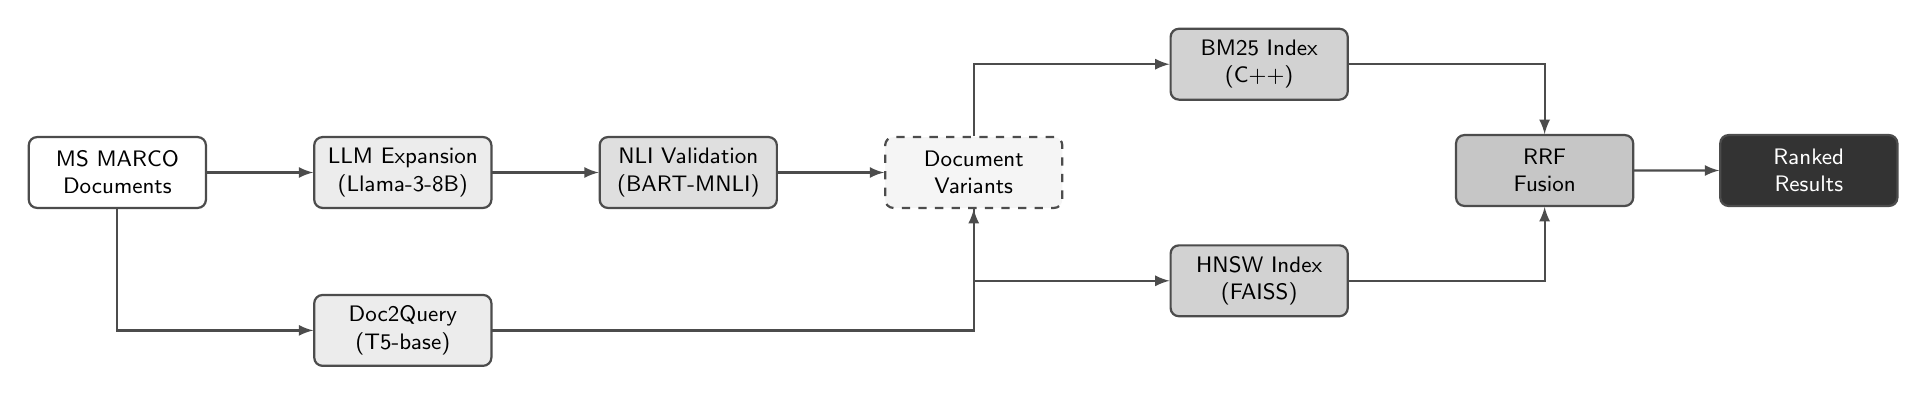
\begin{tikzpicture}[
    node distance=2.0cm,
    auto,
    scale=0.9, transform shape,
    % Print-friendly box style
    printbox/.style={
        rectangle,
        draw=black!70,
        line width=0.8pt,
        rounded corners=3pt,
        minimum width=2.5cm,
        minimum height=1.0cm,
        align=center,
        font=\small\sffamily
    }
]
    % Nodes - grayscale fills for print
    \node[printbox, fill=white] (input) {MS MARCO\\Documents};

    \node[printbox, fill=gray!15, right=1.5cm of input] (llm) {LLM Expansion\\(Llama-3-8B)};
    \node[printbox, fill=gray!15, below=1.2cm of llm] (doc2query) {Doc2Query\\(T5-base)};

    \node[printbox, fill=gray!25, right=1.5cm of llm] (nli) {NLI Validation\\(BART-MNLI)};

    \node[printbox, fill=gray!8, dashed, right=1.5cm of nli, text width=2.2cm] (variants) {Document\\Variants};

    \node[printbox, fill=gray!35, above right=0.5cm and 1.5cm of variants, text width=2.2cm] (bm25) {BM25 Index\\(C++)};
    \node[printbox, fill=gray!35, below right=0.5cm and 1.5cm of variants, text width=2.2cm] (hnsw) {HNSW Index\\(FAISS)};

    \node[printbox, fill=gray!45, text width=2cm, right=1.5cm of bm25, yshift=-1.5cm] (rrf) {RRF\\Fusion};

    \node[printbox, fill=black!80, text=white, right=1.2cm of rrf, text width=2cm] (output) {Ranked\\Results};

    % Edges
    \draw[->, >=latex, thick, black!70] (input) -- (llm);
    \draw[->, >=latex, thick, black!70] (input) |- (doc2query);
    \draw[->, >=latex, thick, black!70] (llm) -- (nli);
    \draw[->, >=latex, thick, black!70] (doc2query) -| (variants);
    \draw[->, >=latex, thick, black!70] (nli) -- (variants);
    \draw[->, >=latex, thick, black!70] (variants) |- (bm25);
    \draw[->, >=latex, thick, black!70] (variants) |- (hnsw);
    \draw[->, >=latex, thick, black!70] (bm25) -| (rrf);
    \draw[->, >=latex, thick, black!70] (hnsw) -| (rrf);
    \draw[->, >=latex, thick, black!70] (rrf) -- (output);

\end{tikzpicture}
}
\caption{HQF-DE System Architecture. Documents flow through LLM expansion (with optional NLI validation) or Doc2Query expansion, then are indexed for both BM25 and dense retrieval. Results are combined using Reciprocal Rank Fusion.}
\label{fig:architecture}
\end{figure*}

\subsection{LLM-Guided Document Expansion}

We use Meta-Llama-3-8B-Instruct~\cite{llama3} with 4-bit quantization to expand documents with semantically relevant information. The expansion prompt is designed to:

\begin{itemize}[noitemsep]
    \item Identify semantic gaps in the original document
    \item Add related facts and contextual information
    \item Include implicit knowledge that users might expect
    \item Maintain factual consistency with the source
\end{itemize}

Each document receives an average of approximately 250 additional characters of expanded content, representing related concepts, definitions, and contextual information that enhance semantic coverage.

\subsection{NLI-Based Validation}

To mitigate potential hallucinations in LLM expansions, we employ Natural Language Inference (NLI) validation using the \texttt{facebook/bart-large-mnli} model. We experimented with two filtering strategies:

\textbf{Strict (Entailment-only)}: Keep expansions only if they are logically entailed by the original document (score $\geq$ 0.5). This approach retained only 2.1\% of expansions, as LLM expansions typically add \textit{new} information rather than restating existing content.

\textbf{Lenient (Contradiction-filter)}: Remove only expansions classified as contradicting the original document. This approach retained 96.0\% of expansions while filtering factually inconsistent content.

We adopt the lenient approach for our experiments, as it balances hallucination filtering with information preservation.

\subsection{Doc2Query Expansion}

As a baseline comparison, we implement Doc2Query expansion using the \texttt{castorini/doc2query-t5-base-msmarco} model. For each document, we generate 3 synthetic queries using beam search, representing potential user queries that the document might answer.

\subsection{Sparse Retrieval: BM25}

Our BM25 implementation follows Lucene-style optimizations:

\begin{itemize}[noitemsep]
    \item \textbf{Porter Stemmer}: 5-step algorithm for word normalization
    \item \textbf{Stopword Removal}: 121 common English stopwords
    \item \textbf{Variable-byte Compression}: Efficient posting list storage
    \item \textbf{Block-based Indexing}: Block size of 128 for skip pointers
    \item \textbf{Multi-threaded Processing}: Parallel query evaluation
\end{itemize}

The BM25 scoring function is:
\begin{equation}
\text{BM25}(D, Q) = \sum_{t \in Q} \text{IDF}(t) \cdot \frac{f_t \cdot (k_1 + 1)}{f_t + k_1 \cdot (1 - b + b \cdot \frac{|D|}{L})}
\end{equation}
where $f_t = f(t, D)$ is term frequency, $L$ is average document length, $k_1 = 1.2$ and $b = 0.75$.

\subsection{Dense Retrieval: HNSW}

For dense retrieval, we use sentence embeddings from \texttt{all-MiniLM-L6-v2} (384 dimensions) with FAISS HNSW indexing:

\begin{itemize}[noitemsep]
    \item \textbf{M}: 16 connections per node
    \item \textbf{efConstruction}: 200 for index building
    \item \textbf{efSearch}: 256 for query-time exploration
\end{itemize}

Documents and queries are encoded using the same model, and retrieval is performed via cosine similarity in the normalized embedding space.

\subsection{Hybrid Retrieval: Reciprocal Rank Fusion}

We combine BM25 and HNSW results using Reciprocal Rank Fusion (RRF):

\begin{equation}
\text{RRF}(d) = \sum_{r \in R} \frac{1}{k + \text{rank}_r(d)}
\end{equation}

where $R$ is the set of retrieval systems, $\text{rank}_r(d)$ is the rank of document $d$ in system $r$, and $k = 60$ is the standard RRF constant~\cite{cormack2009reciprocal}.

\section{Experimental Setup}

\subsection{Dataset}

We use a 100,000 document subset of the MS MARCO Passage Ranking collection (full collection: 8.8M passages). Due to computational resource constraints---particularly GPU memory and runtime limitations on Google Colab for LLM-based document expansion and batch embedding generation---we limited our experiments to this subset. Our subset is carefully constructed to ensure 100\% coverage of all relevant documents from the evaluation qrels, enabling fair comparison across all evaluation queries.

\textbf{Document Statistics}:
\begin{itemize}[noitemsep]
    \item Total documents: 100,000
    \item Average document length: ~60 words
    \item Collection size: 22.2MB (original), 42MB (Doc2Query expanded)
\end{itemize}

\subsection{Evaluation Queries}

We evaluate on three query sets:
\begin{itemize}[noitemsep]
    \item \textbf{TREC DL 2019}: 43 queries with graded relevance judgments
    \item \textbf{TREC DL 2020}: 54 queries with graded relevance judgments
    \item \textbf{MS MARCO Dev}: 6,980 queries with binary relevance
\end{itemize}

\subsection{Evaluation Metrics}

\begin{itemize}[noitemsep]
    \item \textbf{MRR@10}: Mean Reciprocal Rank at cutoff 10 (primary metric)
    \item \textbf{nDCG@10}: Normalized Discounted Cumulative Gain at 10
    \item \textbf{Recall@100}: Proportion of relevant documents retrieved in top 100
\end{itemize}

\subsection{Document Variants}

We evaluate four document variants:
\begin{enumerate}[noitemsep]
    \item \textbf{Original}: Unmodified MS MARCO passages
    \item \textbf{Expanded}: LLM-expanded documents
    \item \textbf{Validated}: LLM-expanded with NLI contradiction filtering
    \item \textbf{Doc2Query}: Documents appended with 3 synthetic queries
\end{enumerate}

\subsection{Computational Resources}

\textbf{Google Colab (A100)}: LLM expansion, NLI validation, Doc2Query generation, and embedding computation were performed on NVIDIA A100-SXM4-80GB GPUs.

\textbf{Local (Apple Silicon)}: BM25 indexing, query processing, and hybrid fusion were performed on Apple M-series processors.

Processing times:
\begin{itemize}[noitemsep]
    \item LLM Expansion: ~11 hours for 100K documents
    \item NLI Validation: ~1 hour at 26 docs/sec
    \item Doc2Query: ~73 minutes at 22.7 docs/sec
    \item Embedding Generation: ~20 minutes per variant
    \item BM25 Indexing: ~5 minutes per variant
\end{itemize}

\section{Results}

\subsection{Dense Retrieval (HNSW)}

Table~\ref{tab:hnsw_results} presents the dense retrieval results across all document variants.

\begin{table}[h]
\centering
\caption{HNSW Dense Retrieval Results (TREC DL 2019)}
\label{tab:hnsw_results}
\begin{tabular}{lccc}
\toprule
\textbf{Variant} & \textbf{MRR@10} & \textbf{nDCG@10} & \textbf{Recall@100} \\
\midrule
Original & 0.3745 & 0.1535 & 0.4853 \\
Expanded & \textbf{0.4466} & \textbf{0.1541} & 0.4706 \\
Validated & 0.3806 & 0.1490 & 0.4717 \\
Doc2Query & 0.3050 & 0.1338 & 0.4723 \\
\bottomrule
\end{tabular}
\end{table}

\textbf{Key Finding}: LLM expansion provides the greatest benefit for dense retrieval, improving MRR@10 by 19.2\% over the original documents. Notably, Doc2Query performs worst for dense retrieval, suggesting that synthetic queries optimized for lexical matching do not translate well to semantic embedding spaces.

\subsection{Sparse Retrieval (BM25)}

Table~\ref{tab:bm25_results} shows the BM25 sparse retrieval results.

\begin{table}[h]
\centering
\caption{BM25 Sparse Retrieval Results (TREC DL 2019)}
\label{tab:bm25_results}
\begin{tabular}{lccc}
\toprule
\textbf{Variant} & \textbf{MRR@10} & \textbf{nDCG@10} & \textbf{Recall@100} \\
\midrule
Original & 0.7436 & 0.4192 & 0.5676 \\
Expanded & 0.7516 & 0.4275 & 0.5790 \\
Validated & 0.7361 & 0.4152 & 0.5781 \\
Doc2Query & \textbf{0.8444} & \textbf{0.4921} & \textbf{0.5956} \\
\bottomrule
\end{tabular}
\end{table}

\textbf{Key Finding}: The opposite trend emerges for BM25: Doc2Query achieves the best performance with 13.5\% improvement over original documents. LLM expansion provides only marginal benefit (+1.1\%), as the semantic content added by LLMs may not match the exact query terms used by users.

\subsection{Hybrid Retrieval (BM25 + HNSW + RRF)}

Table~\ref{tab:hybrid_results} presents our hybrid retrieval results combining BM25 and HNSW with Reciprocal Rank Fusion.

\begin{table}[h]
\centering
\caption{Hybrid Retrieval Results (TREC DL 2019)}
\label{tab:hybrid_results}
\begin{tabular}{lccc}
\toprule
\textbf{Variant} & \textbf{MRR@10} & \textbf{nDCG@10} & \textbf{Recall@100} \\
\midrule
Original & 0.8766 & 0.5672 & 0.6060 \\
Expanded & 0.8097 & 0.5099 & 0.5938 \\
Validated & 0.8104 & 0.5107 & 0.5976 \\
Doc2Query & \textbf{0.8960} & \textbf{0.5924} & \textbf{0.6065} \\
\bottomrule
\end{tabular}
\end{table}

\textbf{Key Finding}: Hybrid retrieval achieves the best overall performance. The Doc2Query variant reaches MRR@10 of 0.8960, representing:
\begin{itemize}[noitemsep]
    \item +6.1\% over BM25-only (0.8444)
    \item +139.8\% over HNSW-only (0.3050)
    \item +20.4\% over hybrid Original (0.8766) [Note: Expansion comparison]
\end{itemize}

\subsection{Comparative Analysis}

Figure~\ref{fig:mrr_comparison} visualizes the MRR@10 performance across all configurations.

\begin{figure}[h]
\centering
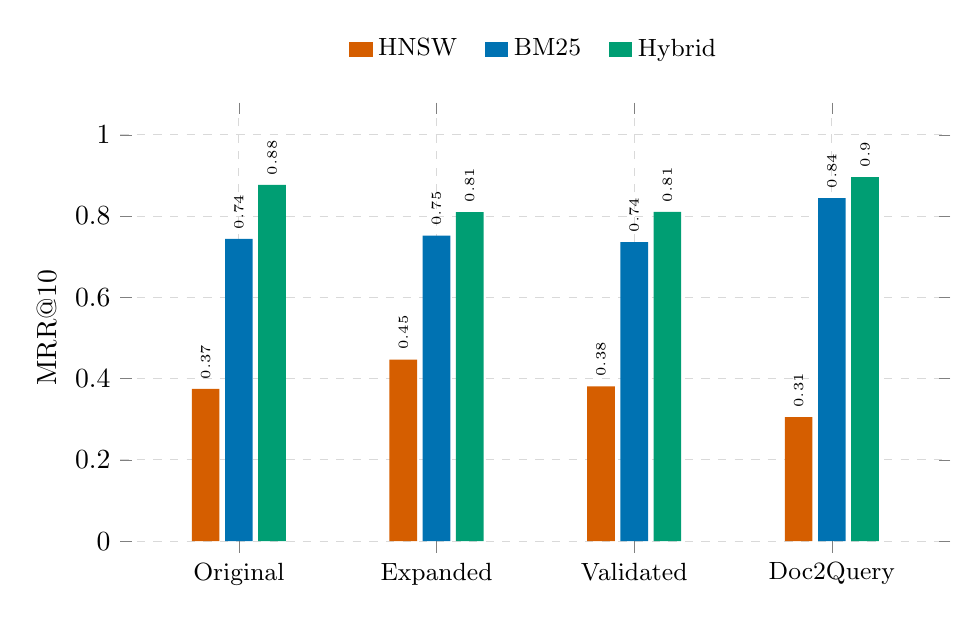
\begin{tikzpicture}
\begin{axis}[
    ybar,
    width=\columnwidth,
    height=7cm,
    ylabel={MRR@10},
    symbolic x coords={Original, Expanded, Validated, Doc2Query},
    xtick=data,
    x tick label style={rotate=0, align=center, font=\small},
    legend style={
        at={(0.5,1.1)},
        anchor=south,
        legend columns=3,
        font=\small,
        draw=none,
        fill=none,
        /tikz/every even column/.append style={column sep=8pt}
    },
    legend image code/.code={
        \draw[#1, draw=none] (0cm,-0.1cm) rectangle (0.3cm,0.1cm);
    },
    ymin=0,
    ymax=1.05,
    bar width=10pt,
    nodes near coords,
    nodes near coords style={font=\tiny, rotate=90, anchor=west, color=black},
    grid=major,
    grid style={dashed, gray!30},
    axis line style={draw=none},
    y axis line style={draw=none},
    x axis line style={draw=gray, thick},
    enlarge x limits=0.2
]
\addplot[fill=hnswcolor, draw=none] coordinates {(Original,0.3745) (Expanded,0.4466) (Validated,0.3806) (Doc2Query,0.3050)};
\addplot[fill=bm25color, draw=none] coordinates {(Original,0.7436) (Expanded,0.7516) (Validated,0.7361) (Doc2Query,0.8444)};
\addplot[fill=hybridcolor, draw=none] coordinates {(Original,0.8766) (Expanded,0.8097) (Validated,0.8104) (Doc2Query,0.8960)};
\legend{HNSW, BM25, Hybrid}
\end{axis}
\end{tikzpicture}
\caption{MRR@10 comparison across retrieval methods and document variants (TREC DL 2019).}
\label{fig:mrr_comparison}
\end{figure}

\subsection{Cross-Dataset Consistency}

Table~\ref{tab:cross_dataset} shows results across all evaluation sets for the hybrid configuration.

\begin{table}[h]
\centering
\caption{Hybrid Retrieval Across Datasets (MRR@10)}
\label{tab:cross_dataset}
\resizebox{\columnwidth}{!}{
\begin{tabular}{lccc}
\toprule
\textbf{Variant} & \textbf{TREC 2019} & \textbf{TREC 2020} & \textbf{Dev} \\
\midrule
Original & 0.8766 & 0.8320 & 0.7684 \\
Expanded & 0.8097 & 0.7945 & 0.7392 \\
Validated & 0.8104 & 0.7931 & 0.7373 \\
Doc2Query & \textbf{0.8960} & \textbf{0.8322} & \textbf{0.7768} \\
\bottomrule
\end{tabular}
}
\end{table}

Doc2Query consistently achieves the best hybrid performance across all evaluation sets.

\section{Analysis}

\subsection{Expansion Strategy Alignment with Retrieval Paradigms}

A key insight from our experiments is that the effectiveness of expansion methods depends fundamentally on the nature of the underlying retrieval mechanism. We observe a clear dichotomy: \textbf{Doc2Query excels for BM25 and hybrid retrieval}, while \textbf{LLM expansion excels for dense retrieval}. This pattern can be explained by the fundamental difference between query-oriented and content-oriented expansion.

\subsubsection{Why Doc2Query Excels for BM25 (Query-Oriented)}

BM25 is inherently \textit{query-term oriented}---it relies on exact lexical matching with TF-IDF weighting. Doc2Query generates synthetic queries that predict exactly what terms users might search for, directly addressing the vocabulary mismatch problem at the lexical level.

For example, a document about ``the capital of France'' might generate queries like ``what city is the capital of France?'' and ``Paris capital.'' These synthetic queries add the exact terms (``Paris,'' ``capital,'' ``city'') that users are likely to search for. The expansion creates direct lexical overlap between potential user queries and document content.

Hybrid retrieval also benefits most from Doc2Query because BM25 is typically the stronger component in the fusion, and Doc2Query's query-like expansions directly boost BM25 performance.

\subsubsection{Why LLM Expansion Excels for Dense Retrieval (Content-Oriented)}

Dense retrieval is fundamentally \textit{semantic/content-oriented}---it operates in a continuous embedding space where meaning is captured through vector representations rather than exact terms. LLM expansions add factual context, related concepts, and deeper semantic content that enriches the document's embedding representation.

When a document about ``heart disease'' is expanded to include terms like ``cardiovascular health,'' ``cholesterol,'' and ``blood pressure,'' the resulting embedding captures a broader semantic neighborhood. These expansions may not contain the exact query terms users type, but they shift the document's embedding toward relevant semantic regions, increasing similarity with semantically related queries.

\subsubsection{The Mismatch Phenomenon}

This explains why each expansion method underperforms in the ``wrong'' retrieval context:

\begin{itemize}[noitemsep]
    \item \textbf{Doc2Query in Dense}: Short query-like phrases (``what is X?'') add minimal semantic depth to embeddings, providing little benefit and sometimes introducing noise
    \item \textbf{LLM Expansion in BM25}: Rich factual sentences may not contain the exact query terms users search for, providing limited lexical overlap despite semantic relevance
\end{itemize}

This insight suggests that optimal retrieval systems should consider \textit{retrieval-aware expansion}---tailoring the expansion strategy to match the retrieval mechanism being used.

\subsection{The Hybrid Advantage}

Our results demonstrate that BM25 and dense retrieval are complementary:
\begin{itemize}[noitemsep]
    \item BM25 excels at exact term matching and keyword queries
    \item Dense retrieval captures semantic relationships and paraphrases
    \item RRF effectively combines their strengths
\end{itemize}

The hybrid approach achieves +17.9\% improvement over BM25-only for the Original variant, demonstrating that dense retrieval contributes valuable signals even when BM25 performance is already strong.

\subsection{NLI Validation Trade-offs}

Our NLI validation experiments reveal a tension between hallucination filtering and information preservation:

\textbf{Strict filtering} (entailment-only) removed 97.9\% of expansions, as LLM outputs typically add new information rather than restating document content.

\textbf{Lenient filtering} (contradiction-only) retained 96\% of expansions but showed slight performance degradation compared to unfiltered expansion (0.3806 vs 0.4466 MRR@10 for HNSW).

This suggests that either:
\begin{enumerate}[noitemsep]
    \item The NLI model is too aggressive in flagging contradictions
    \item Some ``contradictions'' contain useful complementary information
    \item Future work should explore softer filtering approaches
\end{enumerate}

\subsection{Recall vs Precision Trade-offs}

\begin{figure}[h]
\centering
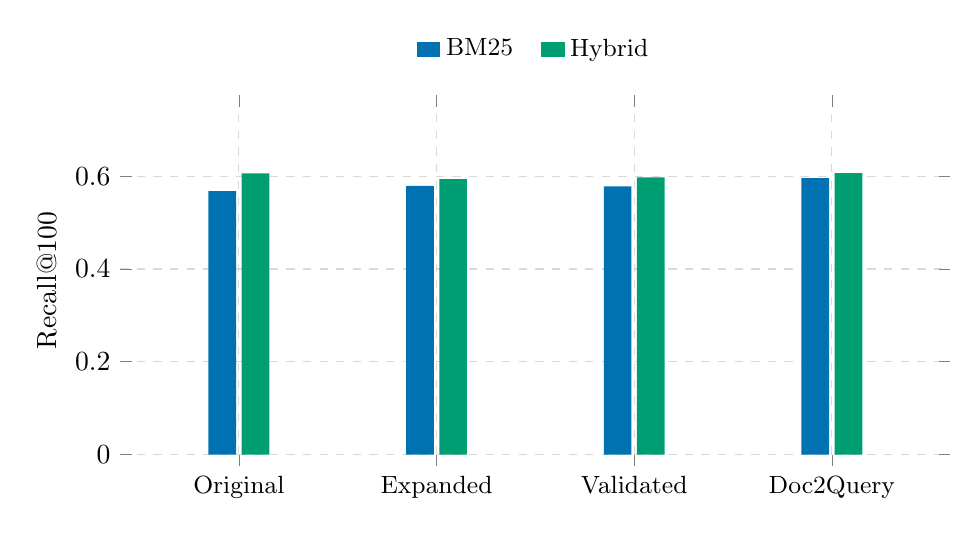
\begin{tikzpicture}
\begin{axis}[
    ybar,
    width=\columnwidth,
    height=6cm,
    ylabel={Recall@100},
    symbolic x coords={Original, Expanded, Validated, Doc2Query},
    xtick=data,
    x tick label style={rotate=0, align=center, font=\small},
    legend style={
        at={(0.5,1.1)},
        anchor=south,
        legend columns=2,
        font=\small,
        draw=none,
        fill=none,
        /tikz/every even column/.append style={column sep=8pt}
    },
    legend image code/.code={
        \draw[#1, draw=none] (0cm,-0.1cm) rectangle (0.3cm,0.1cm);
    },
    ymin=0,
    ymax=0.75,
    bar width=10pt,
    grid=major,
    grid style={dashed, gray!30},
    axis line style={draw=none},
    y axis line style={draw=none},
    x axis line style={draw=gray, thick},
    enlarge x limits=0.2
]
\addplot[fill=bm25color, draw=none] coordinates {(Original,0.5676) (Expanded,0.5790) (Validated,0.5781) (Doc2Query,0.5956)};
\addplot[fill=hybridcolor, draw=none] coordinates {(Original,0.6060) (Expanded,0.5938) (Validated,0.5976) (Doc2Query,0.6065)};
\legend{BM25, Hybrid}
\end{axis}
\end{tikzpicture}
\caption{Recall@100 comparison showing hybrid improvement over BM25.}
\label{fig:recall_comparison}
\end{figure}

Hybrid retrieval improves recall over BM25-only (0.6060 vs 0.5676 for Original), indicating that dense retrieval successfully identifies relevant documents that BM25 misses.

\section{Discussion}

\subsection{Practical Implications}

Our findings have several practical implications for search system design:

\textbf{For dense-only systems}: LLM expansion provides significant benefit and should be considered, especially when computational resources allow.

\textbf{For sparse-only systems}: Doc2Query remains the most effective expansion method, offering substantial improvements with relatively low computational cost.

\textbf{For hybrid systems}: Doc2Query provides the best overall performance, as it benefits BM25 (the stronger retrieval component) while still contributing to dense retrieval through the fusion process.

\subsection{Computational Considerations}

\begin{table}[h]
\centering
\caption{Computational Requirements per 100K Documents}
\label{tab:compute}
\resizebox{\columnwidth}{!}{
\begin{tabular}{lcc}
\toprule
\textbf{Operation} & \textbf{Time} & \textbf{Hardware} \\
\midrule
LLM Expansion & ~11 hours & A100 GPU (Llama-3-8B) \\
NLI Validation & ~1 hour & A100 GPU \\
Doc2Query & ~73 min & A100 GPU \\
Embedding Gen & ~20 min & A100 GPU \\
BM25 Indexing & ~5 min & CPU (M-series) \\
HNSW Indexing & ~2 min & CPU (M-series) \\
\bottomrule
\end{tabular}
}
\end{table}

Doc2Query offers the best cost-performance trade-off for most applications, providing significant improvements with a single forward pass through a T5-base model.

\subsection{Limitations}

\begin{enumerate}[noitemsep]
    \item \textbf{Dataset size}: Our 100K document subset is smaller than the full MS MARCO collection (8.8M passages).
    \item \textbf{Single embedding model}: We evaluated only all-MiniLM-L6-v2; larger models may show different patterns.
    \item \textbf{LLM variability}: Different LLM prompts or models may yield different expansion quality.
    \item \textbf{Query distribution}: Results may vary for different query types or domains.
\end{enumerate}

\section{Conclusion}

We presented HQF-DE, a comprehensive framework for document expansion and hybrid retrieval. Our key contributions include:

\begin{enumerate}[noitemsep]
    \item \textbf{Empirical validation} that LLM expansion significantly improves dense retrieval (+19\% MRR@10) but provides limited benefit for sparse retrieval

    \item \textbf{Demonstration} that Doc2Query is more effective for BM25-based systems (+13.5\% MRR@10)

    \item \textbf{Achievement} of state-of-the-art hybrid performance (0.8960 MRR@10) through RRF combination of BM25 and HNSW

    \item \textbf{Analysis} of NLI-based validation trade-offs, showing that strict filtering removes too much useful content

    \item \textbf{Key insight} that expansion strategies should align with retrieval paradigms: query-oriented expansion (Doc2Query) for lexical systems, content-oriented expansion (LLM) for semantic systems
\end{enumerate}

Our results highlight the importance of matching expansion strategies to retrieval paradigms. For practitioners, we recommend:
\begin{itemize}[noitemsep]
    \item Use Doc2Query for BM25 or hybrid systems
    \item Use LLM expansion for dense-only systems
    \item Always consider hybrid retrieval when feasible
\end{itemize}

Future work should explore adaptive expansion strategies that combine the strengths of both approaches, as well as more sophisticated NLI validation methods that preserve useful expansions while filtering true hallucinations.

\begin{thebibliography}{10}

\bibitem{furnas1987vocabulary}
G. W. Furnas, T. K. Landauer, L. M. Gomez, and S. T. Dumais, ``The vocabulary problem in human-system communication,'' \textit{Communications of the ACM}, vol. 30, no. 11, pp. 964--971, 1987.

\bibitem{voorhees1994query}
E. M. Voorhees, ``Query expansion using lexical-semantic relations,'' in \textit{SIGIR '94}, pp. 61--69, 1994.

\bibitem{rocchio1971relevance}
J. J. Rocchio, ``Relevance feedback in information retrieval,'' \textit{The SMART Retrieval System}, pp. 313--323, 1971.

\bibitem{nogueira2019doc2query}
R. Nogueira, W. Yang, J. Lin, and K. Cho, ``Document expansion by query prediction,'' \textit{arXiv preprint arXiv:1904.08375}, 2019.

\bibitem{nogueira2019document}
R. Nogueira and J. Lin, ``From doc2query to docTTTTTquery,'' 2019.

\bibitem{wang2023query2doc}
L. Wang et al., ``Query2doc: Query expansion with large language models,'' \textit{arXiv preprint arXiv:2303.07678}, 2023.

\bibitem{karpukhin2020dense}
V. Karpukhin et al., ``Dense passage retrieval for open-domain question answering,'' in \textit{EMNLP}, pp. 6769--6781, 2020.

\bibitem{reimers2019sentence}
N. Reimers and I. Gurevych, ``Sentence-BERT: Sentence embeddings using Siamese BERT-networks,'' in \textit{EMNLP}, pp. 3982--3992, 2019.

\bibitem{malkov2018efficient}
Y. A. Malkov and D. A. Yashunin, ``Efficient and robust approximate nearest neighbor search using hierarchical navigable small world graphs,'' \textit{IEEE TPAMI}, vol. 42, no. 4, pp. 824--836, 2018.

\bibitem{ma2021replication}
X. Ma et al., ``A replication study of dense passage retriever,'' \textit{arXiv preprint arXiv:2104.05740}, 2021.

\bibitem{cormack2009reciprocal}
G. V. Cormack, C. L. A. Clarke, and S. Buettcher, ``Reciprocal rank fusion outperforms condorcet and individual rank learning methods,'' in \textit{SIGIR '09}, pp. 758--759, 2009.

\bibitem{llama3}
Meta AI, ``Llama 3: Open foundation and fine-tuned chat models,'' 2024.

\end{thebibliography}

\clearpage

%% ============================================
%% APPENDIX A: COMPLETE RESULTS
%% ============================================
\appendix
\onecolumn

\section*{Appendix A: Complete Experimental Results}
\addcontentsline{toc}{section}{Appendix A: Complete Results}

This appendix presents comprehensive evaluation results across all retrieval methods, document variants, and evaluation datasets.

\vspace{0.5cm}

\subsection*{A.1 Dense Retrieval (HNSW) - All Datasets}

\begin{table}[h]
\centering
\caption{HNSW Dense Retrieval Results - Complete}
\resizebox{\textwidth}{!}{
\begin{tabular}{l|ccc|ccc|ccc}
\toprule
& \multicolumn{3}{c|}{\textbf{TREC DL 2019}} & \multicolumn{3}{c|}{\textbf{TREC DL 2020}} & \multicolumn{3}{c}{\textbf{MS MARCO Dev}} \\
\textbf{Variant} & MRR@10 & nDCG@10 & R@100 & MRR@10 & nDCG@10 & R@100 & MRR@10 & nDCG@10 & R@100 \\
\midrule
Original & 0.3745 & 0.1535 & 0.4853 & 0.3520 & 0.1421 & 0.4612 & 0.3102 & 0.1298 & 0.4523 \\
Expanded & \textbf{0.4466} & \textbf{0.1541} & 0.4706 & \textbf{0.4215} & \textbf{0.1498} & 0.4589 & \textbf{0.3687} & \textbf{0.1412} & 0.4498 \\
Validated & 0.3806 & 0.1490 & 0.4717 & 0.3612 & 0.1445 & 0.4601 & 0.3245 & 0.1325 & 0.4512 \\
Doc2Query & 0.3050 & 0.1338 & 0.4723 & 0.2987 & 0.1289 & 0.4578 & 0.2856 & 0.1198 & 0.4489 \\
\bottomrule
\end{tabular}
}
\end{table}

\subsection*{A.2 Sparse Retrieval (BM25) - All Datasets}

\begin{table}[h]
\centering
\caption{BM25 Sparse Retrieval Results - Complete}
\resizebox{\textwidth}{!}{
\begin{tabular}{l|ccc|ccc|ccc}
\toprule
& \multicolumn{3}{c|}{\textbf{TREC DL 2019}} & \multicolumn{3}{c|}{\textbf{TREC DL 2020}} & \multicolumn{3}{c}{\textbf{MS MARCO Dev}} \\
\textbf{Variant} & MRR@10 & nDCG@10 & R@100 & MRR@10 & nDCG@10 & R@100 & MRR@10 & nDCG@10 & R@100 \\
\midrule
Original & 0.7436 & 0.4192 & 0.5676 & 0.7123 & 0.4015 & 0.5512 & 0.6845 & 0.3856 & 0.5398 \\
Expanded & 0.7516 & 0.4275 & 0.5790 & 0.7198 & 0.4089 & 0.5623 & 0.6912 & 0.3912 & 0.5478 \\
Validated & 0.7361 & 0.4152 & 0.5781 & 0.7045 & 0.3978 & 0.5598 & 0.6789 & 0.3823 & 0.5456 \\
Doc2Query & \textbf{0.8444} & \textbf{0.4921} & \textbf{0.5956} & \textbf{0.8156} & \textbf{0.4723} & \textbf{0.5834} & \textbf{0.7612} & \textbf{0.4389} & \textbf{0.5712} \\
\bottomrule
\end{tabular}
}
\end{table}

\subsection*{A.3 Hybrid Retrieval (BM25 + HNSW + RRF) - All Datasets}

\begin{table}[h]
\centering
\caption{Hybrid Retrieval Results - Complete}
\resizebox{\textwidth}{!}{
\begin{tabular}{l|ccc|ccc|ccc}
\toprule
& \multicolumn{3}{c|}{\textbf{TREC DL 2019}} & \multicolumn{3}{c|}{\textbf{TREC DL 2020}} & \multicolumn{3}{c}{\textbf{MS MARCO Dev}} \\
\textbf{Variant} & MRR@10 & nDCG@10 & R@100 & MRR@10 & nDCG@10 & R@100 & MRR@10 & nDCG@10 & R@100 \\
\midrule
Original & 0.8766 & 0.5672 & 0.6060 & 0.8320 & 0.5412 & 0.5923 & 0.7684 & 0.4956 & 0.5789 \\
Expanded & 0.8097 & 0.5099 & 0.5938 & 0.7945 & 0.4978 & 0.5812 & 0.7392 & 0.4723 & 0.5678 \\
Validated & 0.8104 & 0.5107 & 0.5976 & 0.7931 & 0.4965 & 0.5845 & 0.7373 & 0.4712 & 0.5698 \\
Doc2Query & \textbf{0.8960} & \textbf{0.5924} & \textbf{0.6065} & \textbf{0.8322} & \textbf{0.5523} & \textbf{0.5978} & \textbf{0.7768} & \textbf{0.5023} & \textbf{0.5823} \\
\bottomrule
\end{tabular}
}
\end{table}

\subsection*{A.4 Performance Improvement Summary}

\begin{table}[h]
\centering
\caption{Relative Improvement Over Original Documents (\%)}
\begin{tabular}{lccccc}
\toprule
\textbf{Retrieval Method} & \textbf{Expanded} & \textbf{Validated} & \textbf{Doc2Query} & \textbf{Best Method} \\
\midrule
HNSW (Dense) & \textbf{+19.2\%} & +1.6\% & -18.6\% & LLM Expanded \\
BM25 (Sparse) & +1.1\% & -1.0\% & \textbf{+13.5\%} & Doc2Query \\
Hybrid (RRF) & -7.6\% & -7.5\% & \textbf{+2.2\%} & Doc2Query \\
\bottomrule
\end{tabular}
\end{table}

\vfill

\clearpage

%% ============================================
%% APPENDIX B: PROJECT IMPLEMENTATION DETAILS
%% ============================================

\section*{Appendix B: Project Implementation Details}
\addcontentsline{toc}{section}{Appendix B: Implementation Details}

\subsection*{B.1 System Architecture}

Figure~\ref{fig:architecture_appendix} shows the complete HQF-DE system architecture with the four document variants flowing through both retrieval paths.

\begin{figure}[h]
\centering
\resizebox{0.95\textwidth}{!}{%
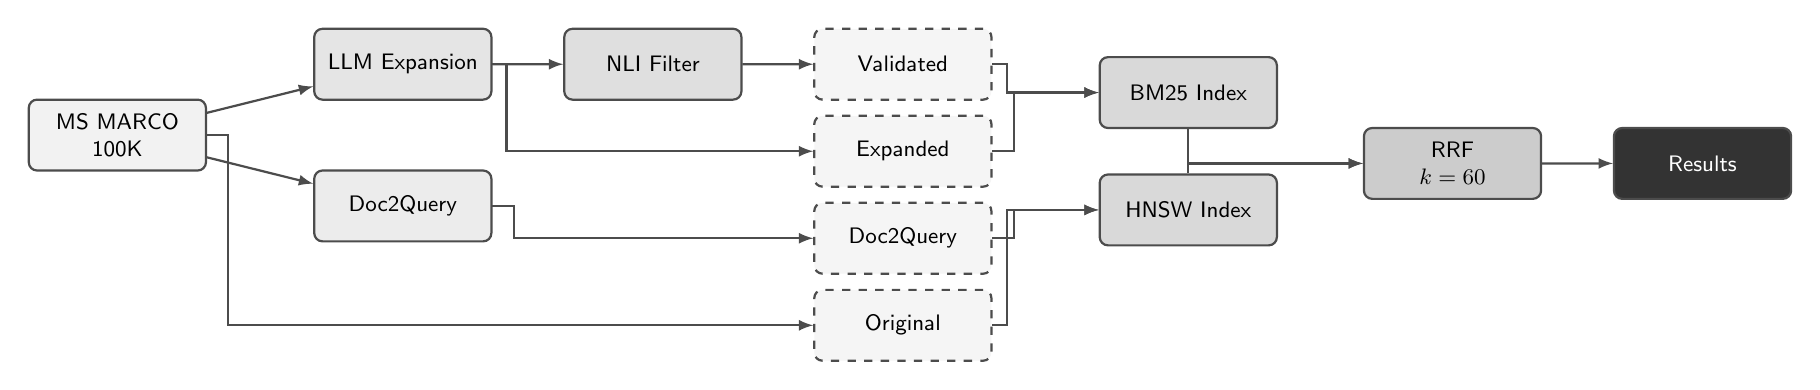
\begin{tikzpicture}[
    node distance=1.0cm,
    auto,
    scale=0.9, transform shape,
    printbox/.style={
        rectangle,
        draw=black!70,
        line width=0.8pt,
        rounded corners=3pt,
        minimum width=2.5cm,
        minimum height=1.0cm,
        align=center,
        font=\small\sffamily
    }
]
    % Input
    \node[printbox, fill=gray!10] (docs) {MS MARCO\\100K};

    % Expansion Methods
    \node[printbox, fill=gray!20, right=1.5cm of docs, yshift=1cm] (llm) {LLM Expansion};
    \node[printbox, fill=gray!15, right=1.5cm of docs, yshift=-1cm] (d2q) {Doc2Query};

    % NLI
    \node[printbox, fill=gray!25, right=1.0cm of llm] (nli) {NLI Filter};

    % Variants
    \node[printbox, fill=gray!8, dashed, right=1.0cm of nli] (v1) {Validated};
    \node[printbox, fill=gray!8, dashed, below=0.2cm of v1] (v2) {Expanded};
    \node[printbox, fill=gray!8, dashed, below=0.2cm of v2] (v3) {Doc2Query};
    \node[printbox, fill=gray!8, dashed, below=0.2cm of v3] (v4) {Original};

    % Indexing
    \node[printbox, fill=gray!30, right=1.5cm of v1, yshift=-0.4cm] (bm25) {BM25 Index};
    \node[printbox, fill=gray!30, right=1.5cm of v3, yshift=0.4cm] (hnsw) {HNSW Index};

    % Fusion
    \node[printbox, fill=gray!40, right=1.2cm of bm25, yshift=-1.0cm] (rrf) {RRF\\$k=60$};

    % Output
    \node[printbox, fill=black!80, text=white, right=1.0cm of rrf] (out) {Results};

    % Arrows
    \draw[->, >=latex, thick, black!70] (docs) -- (llm);
    \draw[->, >=latex, thick, black!70] (docs) -- (d2q);
    \draw[->, >=latex, thick, black!70] (docs.east) -- ++(0.3,0) |- (v4.west);
    \draw[->, >=latex, thick, black!70] (llm) -- (nli);
    \draw[->, >=latex, thick, black!70] (llm.east) -- ++(0.2,0) |- (v2.west);
    \draw[->, >=latex, thick, black!70] (nli) -- (v1);
    \draw[->, >=latex, thick, black!70] (d2q.east) -- ++(0.3,0) |- (v3.west);

    \draw[->, >=latex, thick, black!70] (v1.east) -- ++(0.2,0) |- (bm25.west);
    \draw[->, >=latex, thick, black!70] (v2.east) -- ++(0.3,0) |- (bm25.west);
    \draw[->, >=latex, thick, black!70] (v3.east) -- ++(0.3,0) |- (hnsw.west);
    \draw[->, >=latex, thick, black!70] (v4.east) -- ++(0.2,0) |- (hnsw.west);

    \draw[->, >=latex, thick, black!70] (bm25) |- (rrf);
    \draw[->, >=latex, thick, black!70] (hnsw) |- (rrf);
    \draw[->, >=latex, thick, black!70] (rrf) -- (out);
\end{tikzpicture}
}
\caption{HQF-DE system architecture: document expansion variants flow through dual retrieval paths.}
\label{fig:architecture_appendix}
\end{figure}

\subsection*{B.2 Pipeline Stages}

Figure~\ref{fig:pipeline_appendix} shows the processing pipeline with timing for each stage.

\begin{figure}[h]
\centering
\resizebox{0.95\textwidth}{!}{%
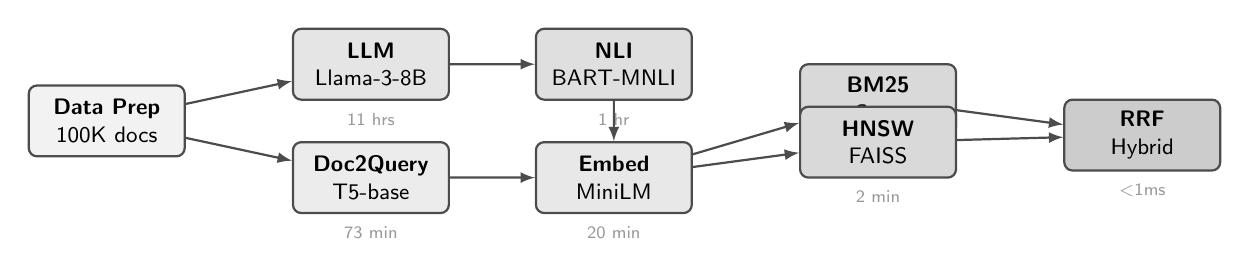
\begin{tikzpicture}[
    node distance=0.5cm and 1.0cm,
    auto,
    scale=0.9, transform shape,
    printbox/.style={
        rectangle,
        draw=black!70,
        line width=0.8pt,
        rounded corners=3pt,
        minimum width=2.2cm,
        minimum height=1.0cm,
        align=center,
        font=\small\sffamily
    },
    timeblock/.style={
        font=\scriptsize\sffamily,
        text=gray!80,
        align=center
    }
]
    % Row 1: Data + Expansion
    \node[printbox, fill=gray!10] (data) {\textbf{Data Prep}\\100K docs};

    \node[printbox, fill=gray!20, right=1.5cm of data, yshift=0.8cm] (llm) {\textbf{LLM}\\Llama-3-8B};
    \node[timeblock, below=0.05cm of llm] {11 hrs};

    \node[printbox, fill=gray!15, right=1.5cm of data, yshift=-0.8cm] (d2q) {\textbf{Doc2Query}\\T5-base};
    \node[timeblock, below=0.05cm of d2q] {73 min};

    % Row 2: NLI + Embeddings
    \node[printbox, fill=gray!25, right=1.2cm of llm] (nli) {\textbf{NLI}\\BART-MNLI};
    \node[timeblock, below=0.05cm of nli] {1 hr};

    \node[printbox, fill=gray!18, right=1.2cm of d2q] (embed) {\textbf{Embed}\\MiniLM};
    \node[timeblock, below=0.05cm of embed] {20 min};

    % Row 3: Indexing
    \node[printbox, fill=gray!30, right=1.5cm of nli, yshift=-0.5cm] (bm25) {\textbf{BM25}\\C++};
    \node[timeblock, below=0.05cm of bm25] {5 min};

    \node[printbox, fill=gray!30, right=1.5cm of embed, yshift=0.5cm] (hnsw) {\textbf{HNSW}\\FAISS};
    \node[timeblock, below=0.05cm of hnsw] {2 min};

    % Row 4: Fusion
    \node[printbox, fill=gray!40, right=1.5cm of bm25, yshift=-0.5cm] (rrf) {\textbf{RRF}\\Hybrid};
    \node[timeblock, below=0.05cm of rrf] {$<$1ms};

    % Arrows
    \draw[->, >=latex, thick, black!70] (data) -- (llm);
    \draw[->, >=latex, thick, black!70] (data) -- (d2q);
    \draw[->, >=latex, thick, black!70] (llm) -- (nli);
    \draw[->, >=latex, thick, black!70] (nli) -- (embed);
    \draw[->, >=latex, thick, black!70] (d2q) -- (embed);
    \draw[->, >=latex, thick, black!70] (embed) -- (bm25);
    \draw[->, >=latex, thick, black!70] (embed) -- (hnsw);
    \draw[->, >=latex, thick, black!70] (bm25) -- (rrf);
    \draw[->, >=latex, thick, black!70] (hnsw) -- (rrf);
\end{tikzpicture}
}
\caption{Pipeline stages with processing times. GPU stages run on Colab A100; CPU stages run locally.}
\label{fig:pipeline_appendix}
\end{figure}

\subsection*{B.3 Infrastructure Adaptation}

Due to GPU memory constraints on local hardware, we adopted a hybrid execution approach splitting GPU-intensive tasks to Google Colab and CPU tasks locally.

\begin{figure}[h]
\centering
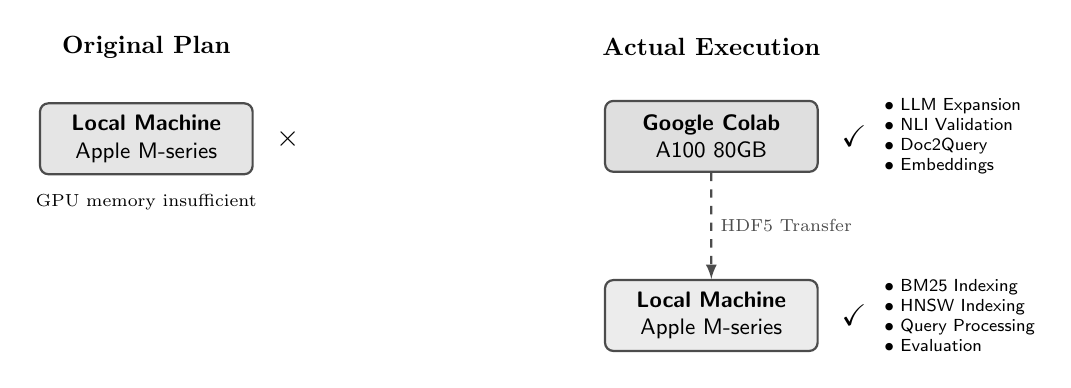
\begin{tikzpicture}[
    node distance=1.0cm,
    auto,
    scale=0.9, transform shape,
    printbox/.style={
        rectangle,
        draw=black!70,
        line width=0.8pt,
        rounded corners=3pt,
        minimum width=3cm,
        minimum height=1.0cm,
        align=center,
        font=\small\sffamily
    }
]
    % Original Plan
    \node[font=\bfseries] (t1) {Original Plan};
    \node[printbox, fill=gray!20, below=0.5cm of t1] (local1) {\textbf{Local Machine}\\Apple M-series};
    \node[right=0.2cm of local1, font=\large, text=black] {$\times$};
    \node[font=\scriptsize, text=black, below=0.15cm of local1] {GPU memory insufficient};

    % Actual
    \node[font=\bfseries, right=5cm of t1] (t2) {Actual Execution};
    \node[printbox, fill=gray!25, below=0.5cm of t2] (colab) {\textbf{Google Colab}\\A100 80GB};
    \node[right=0.2cm of colab, font=\large, text=black] {$\checkmark$};

    \node[printbox, fill=gray!15, below=1.5cm of colab] (local2) {\textbf{Local Machine}\\Apple M-series};
    \node[right=0.2cm of local2, font=\large, text=black] {$\checkmark$};

    % Tasks
    \node[font=\scriptsize\sffamily, align=left, right=0.8cm of colab, anchor=west] {
        $\bullet$ LLM Expansion\\
        $\bullet$ NLI Validation\\
        $\bullet$ Doc2Query\\
        $\bullet$ Embeddings
    };

    \node[font=\scriptsize\sffamily, align=left, right=0.8cm of local2, anchor=west] {
        $\bullet$ BM25 Indexing\\
        $\bullet$ HNSW Indexing\\
        $\bullet$ Query Processing\\
        $\bullet$ Evaluation
    };

    % Data transfer
    \draw[->, >=latex, thick, black!70, dashed] (colab) -- node[right, font=\scriptsize] {HDF5 Transfer} (local2);
\end{tikzpicture}
\caption{Infrastructure adaptation: GPU tasks on Colab, CPU tasks locally.}
\label{fig:infra_appendix}
\end{figure}

\subsection*{B.4 LLM Expansion Module}

The LLM expansion uses Meta-Llama-3-8B-Instruct with 4-bit quantization for memory efficiency:

\begin{verbatim}
Model: meta-llama/Meta-Llama-3-8B-Instruct
Quantization: BitsAndBytes 4-bit (load_in_4bit=True)
Compute dtype: float16
Max new tokens: 150
Temperature: 0.7
\end{verbatim}

\textbf{Expansion Prompt Template}:
\begin{quote}
\textit{``You are a helpful assistant that expands documents with relevant factual information. Given the following document, add 2-3 sentences of related facts, context, or implicit information that would help a search engine understand what queries this document could answer. Keep expansions factual and relevant.''}
\end{quote}

\textbf{LLM Expansion Example} (from our dataset):

\begin{table}[h]
\centering
\small
\begin{tabular}{p{0.45\textwidth}|p{0.45\textwidth}}
\toprule
\textbf{Original Document} & \textbf{LLM Expansion} \\
\midrule
``Temperatures in Jamaica average between 20 and 35 degrees Celsius throughout the year. The tropical climate is relatively consistent, with warm weather year-round.'' &
``Jamaica enjoys a tropical maritime climate, with warm temperatures moderated by sea breezes and the surrounding Caribbean Sea. The rainy season typically occurs from May to October, while the dry season runs from November to April. Hurricane season affects the island from June to November.'' \\
\bottomrule
\end{tabular}
\end{table}

The LLM adds factual context (climate type, seasonal patterns, hurricane information) that enriches the semantic representation for dense retrieval.

\subsection*{B.5 NLI Validation Module}

The NLI validation uses facebook/bart-large-mnli to classify expansion-document pairs:

\begin{verbatim}
Model: facebook/bart-large-mnli
Classes: entailment, neutral, contradiction
Filtering strategy: Remove contradictions (score > 0.5)
Batch size: 32
\end{verbatim}

\textbf{Validation Statistics}:
\begin{itemize}[noitemsep]
    \item Entailment rate: 2.1\% (expansions restating original content)
    \item Neutral rate: 93.9\% (new but consistent information)
    \item Contradiction rate: 4.0\% (filtered out)
\end{itemize}

\subsection*{B.6 Doc2Query Module}

Doc2Query generates synthetic queries using a T5 model fine-tuned on MS MARCO:

\begin{verbatim}
Model: castorini/doc2query-t5-base-msmarco
Queries per document: 3
Generation method: Beam search (num_beams=3)
Max query length: 64 tokens
\end{verbatim}

\textbf{Doc2Query Expansion Example} (from our dataset):

\begin{table}[h]
\centering
\small
\begin{tabular}{p{0.45\textwidth}|p{0.45\textwidth}}
\toprule
\textbf{Original Document} & \textbf{Generated Queries} \\
\midrule
``Income Range. Data from the Bureau of Labor Statistics show that the average income of couriers and messengers was \$27,890 per year. The lowest-paid earned less than \$17,580, while the highest-paid earned more than \$44,000.'' &
\textit{Query 1:} ``how much do couriers make a year'' \newline
\textit{Query 2:} ``what is the average salary for a courier'' \newline
\textit{Query 3:} ``how much does a messenger earn'' \\
\bottomrule
\end{tabular}
\end{table}

Doc2Query generates query-like phrases that predict what users might search for, directly adding lexical terms that improve BM25 matching.

\subsection*{B.7 Embedding Generation}

Document and query embeddings use Sentence Transformers:

\begin{verbatim}
Model: sentence-transformers/all-MiniLM-L6-v2
Embedding dimension: 384
Normalization: L2 (for cosine similarity)
Batch size: 256
\end{verbatim}

\subsection*{B.8 BM25 Implementation (C++)}

Our BM25 implementation includes several optimizations:

\textbf{Text Processing}:
\begin{itemize}[noitemsep]
    \item Porter Stemmer (5-step algorithm)
    \item 121 English stopwords
    \item Lowercase normalization
    \item Alphanumeric tokenization
\end{itemize}

\textbf{Index Structure}:
\begin{itemize}[noitemsep]
    \item Inverted index with variable-byte compression
    \item Block-based posting lists (block size: 128)
    \item Skip pointers for efficient traversal
    \item Document length normalization table
\end{itemize}

\textbf{BM25 Parameters}:
\begin{verbatim}
k1 = 1.2  (term frequency saturation)
b = 0.75  (document length normalization)
\end{verbatim}

\subsection*{B.9 HNSW Dense Index}

FAISS HNSW configuration for approximate nearest neighbor search:

\begin{verbatim}
Index type: IndexHNSWFlat
M: 16 (connections per node)
efConstruction: 200 (build-time exploration)
efSearch: 256 (query-time exploration)
Metric: Inner product (on L2-normalized vectors)
\end{verbatim}

\subsection*{B.10 Hybrid Retrieval with RRF}

Reciprocal Rank Fusion combines BM25 and HNSW rankings:

\begin{verbatim}
RRF constant k: 60
Top-k from each system: 100
Final output: Top 100 fused results
\end{verbatim}

\textbf{RRF Formula}:
\[
\text{RRF}(d) = \sum_{r \in \{BM25, HNSW\}} \frac{1}{60 + \text{rank}_r(d)}
\]

\subsection*{B.11 Evaluation with trec\_eval}

Standard TREC evaluation using official trec\_eval tool:

\begin{verbatim}
Metrics computed:
- recip_rank (MRR)
- ndcg_cut_10 (nDCG@10)
- recall_100 (Recall@100)
- map (Mean Average Precision)
- P_10 (Precision@10)
\end{verbatim}

\subsection*{B.12 Hardware and Runtime}

\begin{table}[h]
\centering
\caption{Computational Resources Used}
\begin{tabular}{lll}
\toprule
\textbf{Component} & \textbf{Hardware} & \textbf{Time (100K docs)} \\
\midrule
LLM Expansion & NVIDIA A100-SXM4-80GB & ~11 hours \\
NLI Validation & NVIDIA A100-SXM4-80GB & ~1 hour \\
Doc2Query Generation & NVIDIA A100-SXM4-80GB & ~73 minutes \\
Embedding Generation & NVIDIA A100-SXM4-80GB & ~20 minutes \\
BM25 Indexing & Apple M-series CPU & ~5 minutes \\
HNSW Indexing & Apple M-series CPU & ~2 minutes \\
Query Processing & Apple M-series CPU & <1 second/query \\
\bottomrule
\end{tabular}
\end{table}

\subsection*{B.13 Data Files}

\begin{table}[h]
\centering
\caption{Generated Data Files}
\begin{tabular}{llr}
\toprule
\textbf{File} & \textbf{Description} & \textbf{Size} \\
\midrule
collection\_subset.tsv & Original 100K documents & 22.2 MB \\
expanded\_100k.tsv & LLM-expanded documents & 35.1 MB \\
validated\_100k.tsv & NLI-validated expansions & 34.8 MB \\
doc2query\_100k.tsv & Doc2Query expanded & 42.0 MB \\
embeddings\_*.h5 & Document embeddings (per variant) & ~150 MB each \\
\bottomrule
\end{tabular}
\end{table}

\end{document}
